%\documentclass[aspectratio=43]{beamer}
\documentclass[c]{beamer}
\usetheme{intridea}  %% Themenwahl

\usepackage[ngerman]{babel} 
\usepackage[T1]{fontenc}    % richtige Silbentrennung
\usepackage[utf8]{inputenc} % Umlaute etc.!
\usepackage{eurosym}
\usepackage{tikz}

\usetikzlibrary{arrows,decorations.pathmorphing,backgrounds,fit,positioning,shapes.symbols,chains}

%1

\title{Freifunk Hamburg}
\author{hamburg.freifunk.net}
\date{2014/Nov/08}

%2
\begin{document}
\maketitle

\begin{frame}{Was ist freifunk?}
	\begin{itemize}
		\item Initiative für freie, offene, kostenlose Netzwerke
		\item Öffentlich - freifunk steht jedem offen, als Nutzer oder Anbieter
		\item Im Besitz der Gemeinschaft - Wird von den Menschen betrieben, die es nutzen
		\item Nicht kommerziell
		\item Ausschliesslich freie, quelloffene Programme
		\item Netzneutral - keine Manipulation der Datenströme
		\item In  \href{http://freifunk.net/wie-mache-ich-mit/community-finden/}{121 Orten} gibt es bereits Freifunknetze mit mehr als 6000 Zugangspunkten
	\end{itemize}
\end{frame}

%3
\begin{frame}{Mit freifunk ins Internet}
	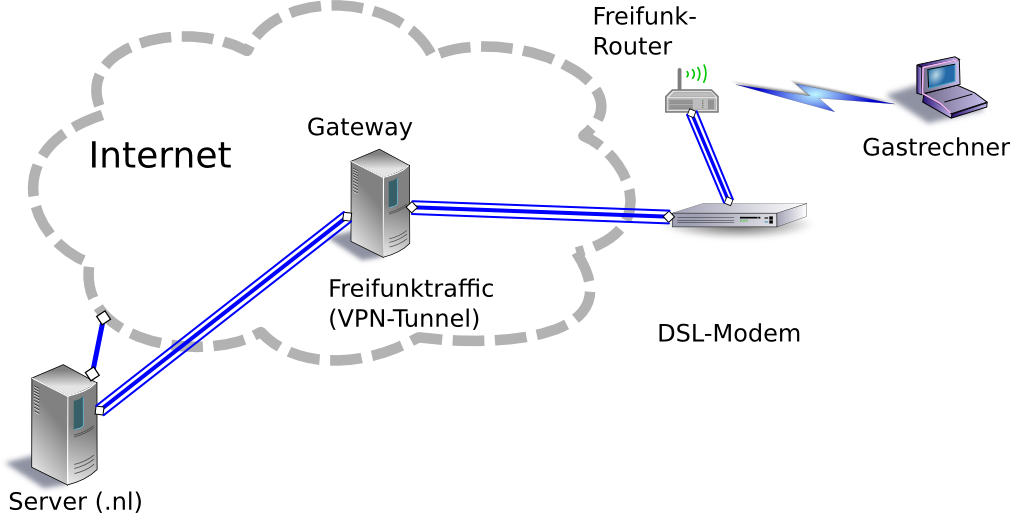
\includegraphics[width=\textwidth]{Bilder/Freifunk_Knotenanbindung}
\end{frame}


%4
\begin{frame}{Mesh}
	Zwei SSIDs
	\begin{itemize}
		\item Freifunk Zugang: hamburg.freifunk.net
		\item Meshing (adhoc): f8:d1:11:87:52:2e
	\end{itemize}
	Was ist ein mesh?
	\begin{itemize}
		\item to mesh = Englisch: vermaschen
		\item Selbst organisierendes Netzwerk
		\item hamburg.freifunk.net nutzt das Protokoll B.A.T.M.A.N.-adv.
	\end{itemize}
\end{frame}


%5
\begin{frame}{Mesh}
	\begin{center}
		\begin{tikzpicture}
			\definecolor{outerCircleColour}{RGB}{220, 0, 103}
			\definecolor{innerCircleColour}{RGB}{255, 203, 18}
			\tikzstyle{vertex}=[circle, draw, color=outerCircleColour, ultra thick, minimum size=84pt]
			\tikzstyle{place}=[circle, draw, color=innerCircleColour, fill=innerCircleColour, minimum size=6pt, inner sep=0pt]

			\node [vertex] (a) {};
			\node [vertex, xshift=68pt, yshift=24pt] (b) {};
			\node [vertex, xshift=112pt, yshift=-20pt] (c) {};

			\node [place, label=above:$A$] (A) {};
			\node [place, xshift=68pt, yshift=24pt, label=above:$B$] (B) {};
			\node [place, xshift=112pt, yshift=-20pt, label=right:$C$] (C) {};

			\path[-, thick, color=gray]
			(A) edge (B)
			(B) edge (C);
		\end{tikzpicture}
	\end{center}
\end{frame}


%6
\begin{frame}{Mesh}
	\begin{center}
		\begin{tikzpicture}
\definecolor{outerCircleColour}{RGB}{220, 0, 103}
			\definecolor{innerCircleColour}{RGB}{255, 203, 18}
			\tikzstyle{vertex}=[circle, draw, color=outerCircleColour, ultra thick, minimum size=84pt]
			\tikzstyle{place}=[circle, draw, color=innerCircleColour, fill=innerCircleColour, minimum size=6pt, inner sep=0pt]

			\node [vertex] (a) {};
			\node [vertex, xshift=68pt, yshift=24pt] (b) {};
			\node [vertex, xshift=112pt, yshift=-20pt] (c) {};

			\node [place, label=above:$A$] (A) {};
			\node [place, xshift=68pt, yshift=24pt, label=above:$B$] (B) {};
			\node [place, xshift=112pt, yshift=-20pt, label=right:$C$] (C) {};

			\path[-, thick, color=gray]
			(A) edge (B)
			(B) edge (C)
			(A) edge[dashed] (C);
		\end{tikzpicture}
	\end{center}
\end{frame}

%7
\begin{frame}{Das Netz wächst}
	\begin{center}
		\begin{tikzpicture}
			\definecolor{outerCircleColour}{RGB}{220, 0, 103}
			\definecolor{innerCircleColour}{RGB}{255, 203, 18}
			\tikzstyle{vertex}=[circle, draw, color=outerCircleColour, ultra thick, minimum size=40pt]
			\tikzstyle{place}=[circle, draw, color=innerCircleColour, fill=innerCircleColour, minimum size=7pt, inner sep=0pt]

			\node [vertex] (a) {};
			\node [vertex, xshift=15pt, yshift=30pt] (b) {};
			\node [vertex, xshift=65pt, yshift=5pt] (c) {};
			\node [vertex, xshift=33pt, yshift=-3pt] (d) {};
			\node [vertex, xshift=85pt, yshift=-25pt] (e) {};
			\node [vertex, xshift=100pt, yshift=2pt] (f) {};
			\node [vertex, xshift=91pt, yshift=32pt] (g) {};
			\node [vertex, xshift=110pt, yshift=-52pt] (h) {};
			\node [vertex, xshift=124pt, yshift=23pt] (i) {};
			\node [vertex, xshift=134pt, yshift=-7pt] (j) {};
			\node [vertex, xshift=164pt, yshift=-14pt] (k) {};
			\node [vertex, xshift=144pt, yshift=-66pt] (l) {};
			\node [vertex, xshift=170pt, yshift=-46pt] (m) {};
			\node [vertex, xshift=201pt, yshift=-59pt] (n) {};

			\node [place] (A) {};
			\node [place, xshift=15pt, yshift=30pt] (B) {};
			\node [place, xshift=65pt, yshift=5pt] (C) {};
			\node [place, xshift=33pt, yshift=-3pt] (D) {};
			\node [place, xshift=85pt, yshift=-25pt] (E) {};
			\node [place, xshift=100pt, yshift=2pt] (F) {};
			\node [place, xshift=91pt, yshift=32pt] (G) {};
			\node [place, xshift=110pt, yshift=-52pt] (H) {};
			\node [place, xshift=124pt, yshift=23pt] (I) {};
			\node [place, xshift=134pt, yshift=-7pt] (J) {};
			\node [place, xshift=164pt, yshift=-14pt] (K) {};
			\node [place, xshift=144pt, yshift=-66pt] (L) {};
			\node [place, xshift=170pt, yshift=-46pt] (M) {};
			\node [place, xshift=201pt, yshift=-59pt] (N) {};

			\path[-, thick, color=gray]
			(A) edge (B)
			(A) edge (D)
			(B) edge (D)
			(C) edge (D)
			(C) edge (E)
			(C) edge (F)
			(C) edge (G)
			(E) edge (F)
			(E) edge (H)
			(F) edge (G)
			(F) edge (I)
			(F) edge (J)
			(G) edge (I)
			(H) edge (L)
			(I) edge (J)
			(J) edge (K)
			(K) edge (M)
			(L) edge (M)
			(M) edge (N);
		\end{tikzpicture}
	\end{center}
\end{frame}


%8
\begin{frame}{Netzwerke verbinden sich untereinander}
	\begin{columns}[c]
		\begin{column}[]{.4\textwidth}
			\scalebox{0.6}[0.6]{
			\begin{tikzpicture}
				\definecolor{outerCircleColour}{RGB}{220, 0, 103}
				\definecolor{innerCircleColour}{RGB}{255, 203, 18}
				\tikzstyle{vertex}=[circle, draw, color=outerCircleColour, ultra thick, minimum size=40pt]
				\tikzstyle{place}=[circle, draw, color=innerCircleColour, fill=innerCircleColour, minimum size=7pt, inner sep=0pt]

				\node [vertex] (a) {};
				\node [vertex, xshift=15pt, yshift=30pt] (b) {};
				\node [vertex, xshift=65pt, yshift=5pt] (c) {};
				\node [vertex, xshift=33pt, yshift=-3pt] (d) {};
				\node [vertex, xshift=85pt, yshift=-25pt] (e) {};
				\node [vertex, xshift=100pt, yshift=2pt] (f) {};
				\node [vertex, xshift=91pt, yshift=32pt] (g) {};
				\node [vertex, xshift=110pt, yshift=-52pt] (h) {};
				\node [vertex, xshift=124pt, yshift=23pt] (i) {};
				\node [vertex, xshift=134pt, yshift=-7pt] (j) {};
				\node [vertex, xshift=164pt, yshift=-14pt] (k) {};
				\node [vertex, xshift=144pt, yshift=-66pt] (l) {};
				\node [vertex, xshift=170pt, yshift=-46pt] (m) {};
				\node [vertex, xshift=201pt, yshift=-59pt] (n) {};

				\node [place] (A) {};
				\node [place, xshift=15pt, yshift=30pt] (B) {};
				\node [place, xshift=65pt, yshift=5pt] (C) {};
				\node [place, xshift=33pt, yshift=-3pt] (D) {};
				\node [place, xshift=85pt, yshift=-25pt] (E) {};
				\node [place, xshift=100pt, yshift=2pt] (F) {};
				\node [place, xshift=91pt, yshift=32pt] (G) {};
				\node [place, xshift=110pt, yshift=-52pt] (H) {};
				\node [place, xshift=124pt, yshift=23pt] (I) {};
				\node [place, xshift=134pt, yshift=-7pt] (J) {};
				\node [place, xshift=164pt, yshift=-14pt] (K) {};
				\node [place, xshift=144pt, yshift=-66pt] (L) {};
				\node [place, xshift=170pt, yshift=-46pt] (M) {};
				\node [place, xshift=201pt, yshift=-59pt] (N) {};

				\path[-, thick, color=gray]
				(A) edge (B)
				(A) edge (D)
				(B) edge (D)
				(C) edge (D)
				(C) edge (E)
				(C) edge (F)
				(C) edge (G)
				(E) edge (F)
				(E) edge (H)
				(F) edge (G)
				(F) edge (I)
				(F) edge (J)
				(G) edge (I)
				(H) edge (L)
				(I) edge (J)
				(J) edge (K)
				(K) edge (M)
				(L) edge (M)
				(M) edge (N);
			\end{tikzpicture}}
		\end{column}
		\begin{column}{0.185\textwidth}
			\begin{uncoverenv}<2->
				\begin{tikzpicture}
					\definecolor{outerCircleColour}{RGB}{220, 0, 103}
					\definecolor{innerCircleColour}{RGB}{255, 203, 18}

					\draw[color=white] (280pt, 85pt) arc (0:0:0pt);
					\draw[color=white] (-180pt, 85pt) arc (0:0:0pt);

					\draw[color=outerCircleColour, thick, xshift=-50pt, yshift=9pt] (-110pt, 0pt) arc (270:450:6pt);
					\draw[color=outerCircleColour, thick, xshift=-50pt, yshift=11pt] (-110pt, 0pt) arc (270:450:4pt);
					\draw[color=outerCircleColour, thick, xshift=-50pt, yshift=13pt] (-110pt, 0pt) arc (270:450:2pt);

					\draw[color=outerCircleColour, thick, xshift=-9pt, yshift=21pt] (-110pt, 0pt) arc (90:270:6pt);
					\draw[color=outerCircleColour, thick, xshift=-9pt, yshift=19pt] (-110pt, 0pt) arc (90:270:4pt);
					\draw[color=outerCircleColour, thick, xshift=-9pt, yshift=17pt] (-110pt, 0pt) arc (90:270:2pt);

					\draw[color=gray, ultra thick, xshift=-50pt, yshift=15] (-103pt, 0pt) edge[dashed] (-74pt, 0pt);
				\end{tikzpicture}
			\end{uncoverenv}
		\end{column}
		\begin{column}[]{.5\textwidth}
			\reflectbox{
			\scalebox{0.6}[0.6]{
			\begin{tikzpicture}
				\definecolor{outerCircleColour}{RGB}{220, 0, 103}
				\definecolor{innerCircleColour}{RGB}{255, 203, 18}
				\tikzstyle{vertex}=[circle, draw, color=outerCircleColour, ultra thick, minimum size=40pt]
				\tikzstyle{place}=[circle, draw, color=innerCircleColour, fill=innerCircleColour, minimum size=7pt, inner sep=0pt]

				\node [vertex] (a) {};
				\node [vertex, xshift=15pt, yshift=30pt] (b) {};
				\node [vertex, xshift=65pt, yshift=5pt] (c) {};
				\node [vertex, xshift=33pt, yshift=-3pt] (d) {};
				\node [vertex, xshift=85pt, yshift=-25pt] (e) {};
				\node [vertex, xshift=100pt, yshift=2pt] (f) {};
				\node [vertex, xshift=91pt, yshift=32pt] (g) {};
				\node [vertex, xshift=110pt, yshift=-52pt] (h) {};
				\node [vertex, xshift=124pt, yshift=23pt] (i) {};
				\node [vertex, xshift=134pt, yshift=-7pt] (j) {};
				\node [vertex, xshift=164pt, yshift=-14pt] (k) {};
				\node [vertex, xshift=144pt, yshift=-66pt] (l) {};
				\node [vertex, xshift=170pt, yshift=-46pt] (m) {};
				\node [vertex, xshift=201pt, yshift=-59pt] (n) {};

				\node [place] (A) {};
				\node [place, xshift=15pt, yshift=30pt] (B) {};
				\node [place, xshift=65pt, yshift=5pt] (C) {};
				\node [place, xshift=33pt, yshift=-3pt] (D) {};
				\node [place, xshift=85pt, yshift=-25pt] (E) {};
				\node [place, xshift=100pt, yshift=2pt] (F) {};
				\node [place, xshift=91pt, yshift=32pt] (G) {};
				\node [place, xshift=110pt, yshift=-52pt] (H) {};
				\node [place, xshift=124pt, yshift=23pt] (I) {};
				\node [place, xshift=134pt, yshift=-7pt] (J) {};
				\node [place, xshift=164pt, yshift=-14pt] (K) {};
				\node [place, xshift=144pt, yshift=-66pt] (L) {};
				\node [place, xshift=170pt, yshift=-46pt] (M) {};
				\node [place, xshift=201pt, yshift=-59pt] (N) {};

				\path[-, thick, color=gray]
				(A) edge (B)
				(A) edge (D)
				(B) edge (D)
				(C) edge (D)
				(C) edge (E)
				(C) edge (F)
				(C) edge (G)
				(E) edge (F)
				(E) edge (H)
				(F) edge (G)
				(F) edge (I)
				(F) edge (J)
				(G) edge (I)
				(H) edge (L)
				(I) edge (J)
				(J) edge (K)
				(K) edge (M)
				(L) edge (M)
				(M) edge (N);
			\end{tikzpicture}}}
		\end{column}
	\end{columns}
\end{frame}


%9
\begin{frame}{Demo}
	\begin{itemize}
		\item Knotenkarte \href{http://knotenkarte.de}{http://knotenkarte.de}
	\end{itemize}
\end{frame}




%10
\begin{frame}{Sicherheit}
	\begin{itemize}
		\item Da freifunk kein Kennwort nutzt, ist die Funkstrecke zum Zugangspunkt (wie bei allen offenen WLANs) unverschlüsselt
		\item Wie sonst im Netz auch, nutzt nach Möglichkeit Ende-zu-Ende-Verschlüsselung
		\item Verbindung freifunk-Knoten zu Gateway läuft durch VPN und ist verschlüsselt --> kein Zugriff auf das „Heimnetzwerk“ möglich
	\end{itemize}
\end{frame}


%11
\begin{frame}{Störerhaftung}
	\begin{itemize}
		\item Die Zugangspunkte gehen nicht direkt in das Internet
		\item Es wird über das Internet eine verschlüsselte VPN-Verbindung zu den Gateways aufgebaut
		\item Selbst die Gateways sind nicht die Ausgänge ins GBI, sondern bauen wiederum VPNs ins Ausland auf
	\end{itemize}
\end{frame}


%12
\begin{frame}{Dienste}
	Implementiert
	\begin{itemize}
		\item Internet (IPv4 \& IPv6)
		\item Stadtweites Intranet (IPv4 \& IPv6)
		\item Internet Dienste \href{http://hamburg.freifunk.net/wo-wird-gefunkt\#Dienste}{http://hamburg.freifunk.net/wo-wird-gefunkt\#Dienste}
		\item Verbindungen zu anderen Städten und Netzwerken sowie deren Diensten
	\end{itemize}
\end{frame}

%13
\begin{frame}{Richtfunknetz}
	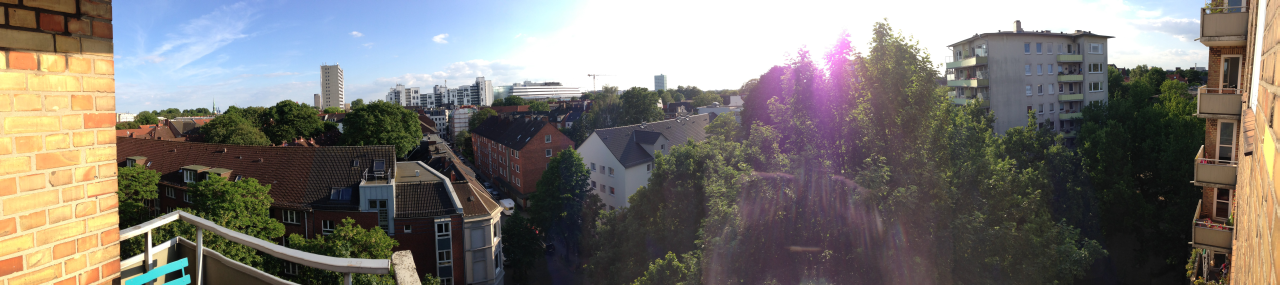
\includegraphics[width=\textwidth]{Bilder/esmarch95}
	\begin{columns}
		\begin{column}{0.7\textwidth}
			\begin{itemize}
				\item Heute wird Verbund der Stadteile über VPN-Tunnel durch das Internet realisiert (Abhängigkeit vom Internet und zentraler Gateways)
				\item Eine Alternative bietet der Aufbau einer eigenen Infrastruktur mit Richtfunkstrecken von Dach zu Dach
			\end{itemize}
		\end{column}
		\begin{column}{0.3\textwidth}
			\begin{center}
				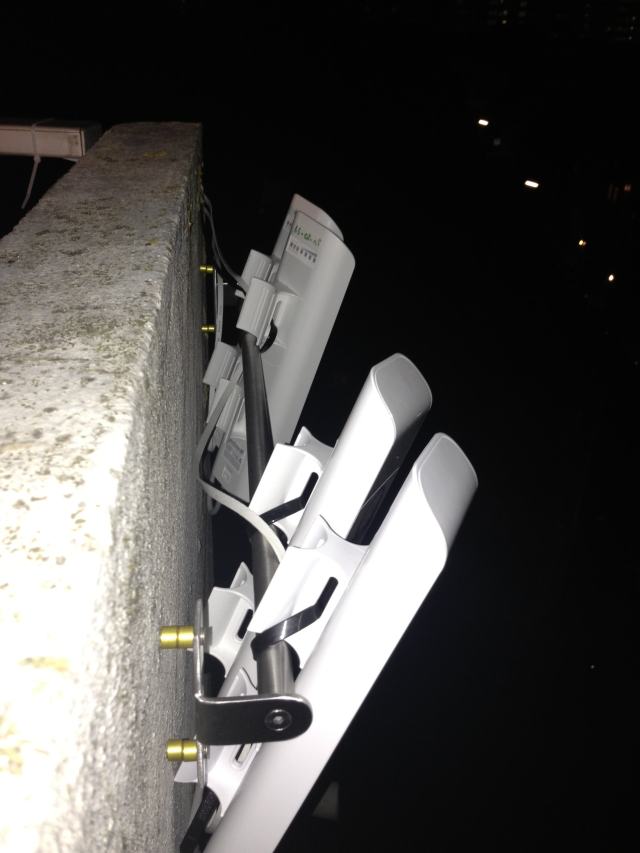
\includegraphics[width=.8\textwidth]{Bilder/esmarch95-2}
			\end{center}
		\end{column}
	\end{columns}
	
\end{frame}


%14
\begin{frame}{Wie kann man mitmachen?}
	\begin{itemize}
		\item Alle können Freifunker\textunderscore innen werden, besondere technische Kenntnisse sind nicht erforderlich
		\item Werde ein Teil des Netzwerks, indem du bei dir im Haus einen Freifunk-Knoten aufstellst
		\item Treffen jeden Montag ab 19:00 Uhr in den Rämen des CCCHH, Freitags ab 19:30 Uhr im Attraktor
	\end{itemize}
\end{frame}


%15
\begin{frame}{Helft mit!}
	\begin{itemize}
		\item \href{http://www.ohrensessel.net/ffhh/graph/total/year}{Stellt mehr Knoten auf}
		\item \href{http://media.hamburg.freifunk.net}{Macht graphische Gestaltung}
		\item Organisiert mit
		\item Betreibt Öffentlichkeitsarbeit
		\item \href{http://hamburg.freifunk.net/wo-wird-gefunkt\#Dienste}{Bietet eigene Dienste an}
		\item Verbreitet die Idee
	\end{itemize}
\end{frame}


%16
\begin{frame}{Entwickelt mit!}
	\begin{itemize}
		\item \href{http://hamburg.freifunk.net}{Verbessert die Seite}
		\item \href{http://knotenkarte.de}{Fügt der Knotenkarte neue Fähigkeiten hinzu}
		\item \href{http://www.ohrensessel.net/ffhh/total}{Bohrt die Statistiken auf (gamification)}
		\item \href{https://github.com/freifunkhamburg/}{Entwickelt firmware}
		\item \href{http://wiki.freifunk.net/Freifunk_Hamburg\#Technik}{Helft das Netz zu administrieren}
	\end{itemize}
\end{frame}


%17
\begin{frame}{Vielen Dank!}
	\begin{columns}
		\begin{column}{0.6\textwidth}
			\begin{itemize}
				\item Netz: hamburg.freifunk.net
				\item Mail: kontakt@hamburg.freifunk.net
		\end{itemize}
		\end{column}
		\begin{column}{0.4\textwidth}
			\begin{center}
				
\includegraphics[width=0.5\textwidth]{Bilder/cc-by}
			\end{center}
		\end{column}
	\end{columns}
\end{frame}

\end{document}